\documentclass{beamer}

\usecolortheme{orchid}

\usefonttheme[onlymath]{serif}
%Information to be included in the title page:
\title{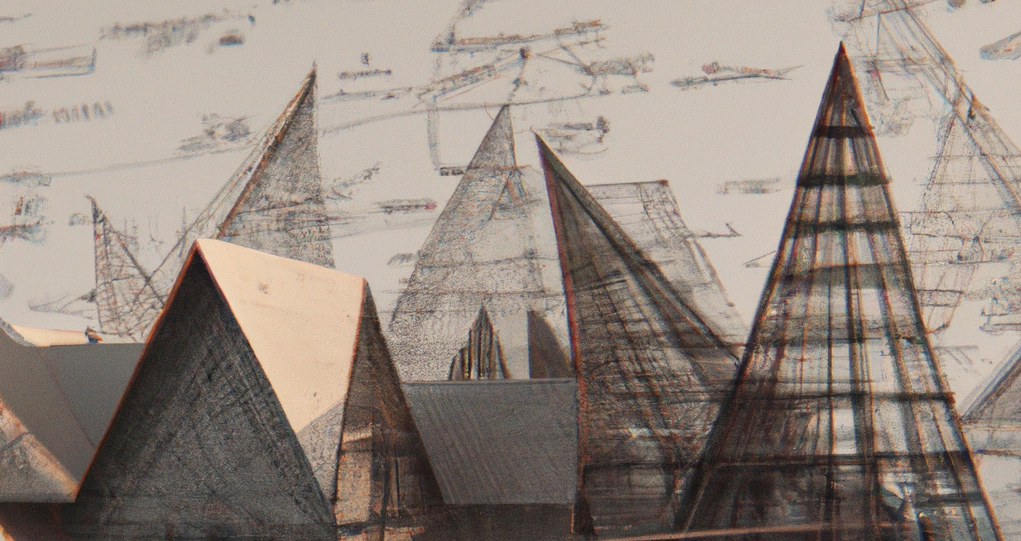
\includegraphics[width=12em]{FallingRoofs1.png}\\Computation in logic as the splitting of idempotents in algebraic geometry;\\ two models of multiplicative linear logic.}
\author{Daniel Murfet, William Troiani}
\institute{University of Melbourne, University of Sorbonne Paris Nord}
\date{2022}

\setbeamercolor{background canvas}{bg=gray!20}

\usepackage{amsthm}
\usepackage{amsmath}
\usepackage{amsfonts}
\usepackage{algorithm}
\usepackage{mathrsfs}
\usepackage{array}
\usepackage{amssymb}
\usepackage{units}
\usepackage{graphicx}
\usepackage{tikz-cd}
\usepackage{nicefrac}
\usepackage{hyperref}
\usepackage{bbm}
\usepackage{color}
\usepackage{tensor}
\usepackage{tipa}
\usepackage{bussproofs}
\usepackage{ stmaryrd }
\usepackage{ textcomp }
\usepackage{leftidx}
\usepackage{afterpage}
\usepackage{varwidth}
\usepackage{tasks}
\usepackage{ cmll }
\usepackage{makecell}
\usepackage{MnSymbol}
\usepackage{quiver}
\usepackage{adjustbox}
\usepackage{multirow}
\usepackage{booktabs}
\usepackage{xparse}
\usepackage{calc}
\usepackage{braket}

\newcommand\blankpage{
	\null
	\thispagestyle{empty}
	\addtocounter{page}{-1}
	\newpage
}

\graphicspath{ {images/} }

\theoremstyle{plain}
\newtheorem{thm}{Theorem}[subsection] % reset theorem numbering for each chapter
\newtheorem{proposition}[thm]{Proposition}
%\newtheorem{lemma}[thm]{Lemma}
%\newtheorem{fact}[thm]{Fact}
\newtheorem{cor}[thm]{Corollary}

\theoremstyle{definition}
\newtheorem{defn}[thm]{Definition} % definition numbers are dependent on theorem numbers
\newtheorem{exmp}[thm]{Example} % same for example numbers
\newtheorem{notation}[thm]{Notation}
\newtheorem{remark}[thm]{Remark}
\newtheorem{condition}[thm]{Condition}
\newtheorem{question}[thm]{Question}
\newtheorem{construction}[thm]{Construction}
\newtheorem{exercise}[thm]{Exercise}
%\newtheorem{example}[thm]{Example}
\newtheorem{aside}[thm]{Aside}

\def\doubleunderline#1{\underline{\underline{#1}}}
\newcommand{\bb}[1]{\mathbb{#1}}
\newcommand{\scr}[1]{\mathscr{#1}}
\newcommand{\call}[1]{\mathcal{#1}}
\newcommand{\psheaf}{\text{\underline{Set}}^{\scr{C}^{\text{op}}}}
\newcommand{\und}[1]{\underline{\hspace{#1 cm}}}
\newcommand{\adj}[1]{\text{\textopencorner}{#1}\text{\textcorner}}
\newcommand{\comment}[1]{}
\newcommand{\lto}{\longrightarrow}
\newcommand{\rone}{(\operatorname{R}\bold{1})}
\newcommand{\lone}{(\operatorname{L}\bold{1})}
\newcommand{\rimp}{(\operatorname{R} \multimap)}
\newcommand{\limp}{(\operatorname{L} \multimap)}
\newcommand{\rtensor}{(\operatorname{R}\otimes)}
\newcommand{\ltensor}{(\operatorname{L}\otimes)}
\newcommand{\rtrue}{(\operatorname{R}\top)}
\newcommand{\rwith}{(\operatorname{R}\\&)}
\newcommand{\lwithleft}{(\operatorname{L}\\&)_{\operatorname{left}}}
\newcommand{\lwithright}{(\operatorname{L}\\&)_{\operatorname{right}}}
\newcommand{\rplusleft}{(\operatorname{R}\oplus)_{\operatorname{left}}}
\newcommand{\rplusright}{(\operatorname{R}\oplus)_{\operatorname{right}}}
\newcommand{\lplus}{(\operatorname{L}\oplus)}
\newcommand{\prom}{(\operatorname{prom})}
\newcommand{\ctr}{(\operatorname{ctr})}
\newcommand{\der}{(\operatorname{der})}
\newcommand{\weak}{(\operatorname{weak})}
\newcommand{\exi}{(\operatorname{exists})}
\newcommand{\fa}{(\operatorname{for\text{ }all})}
\newcommand{\ex}{(\operatorname{ex})}
\newcommand{\cut}{(\operatorname{cut})}
\newcommand{\ax}{(\operatorname{ax})}
\newcommand{\negation}{\sim}
\newcommand{\true}{\top}
\newcommand{\false}{\bot}
\DeclareRobustCommand{\diamondtimes}{%
	\mathbin{\text{\rotatebox[origin=c]{45}{$\boxplus$}}}%
}
\newcommand{\tagarray}{\mbox{}\refstepcounter{equation}$(\theequation)$}
\newcommand{\startproof}[1]{
	\AxiomC{#1}
	\noLine
	\UnaryInfC{$\vdots$}
}
\newenvironment{scprooftree}[1]%
{\gdef\scalefactor{#1}\begin{center}\proofSkipAmount \leavevmode}%
	{\scalebox{\scalefactor}{\DisplayProof}\proofSkipAmount \end{center} }
\newcommand\Wider[2][3em]{%
	\makebox[\linewidth][c]{%
		\begin{minipage}{\dimexpr\textwidth+#1\relax}
			\raggedright#2
		\end{minipage}%
	}%
}
% https://tex.stackexchange.com/questions/63355/wrapping-cmidrule-in-a-macro
\ExplSyntaxOn
\makeatletter
\newcommand{\CMidRule}{\noalign\bgroup\@CMidRule{}}
\NewDocumentCommand{\@CMidRule}{
	m % Material to reinsert before cmidrule.
	O{0.0ex} % #1 = left adjust
	O{0.0ex} % #1 = right adjust
	m  %       #3 = columns to span
}{
	\peek_meaning_remove_ignore_spaces:NTF \CMidRule
	{ \@CMidRule { #1 \cmidrule[\cmidrulewidth](l{#2}r{#3}){#4} } }
	{ \egroup #1 \cmidrule[\cmidrulewidth](l{#2}r{#3}){#4} }
}
\makeatother
\ExplSyntaxOff

\newcommand{\PhantC}{\phantom{\colon}}%
\newcommand{\PhantSQ}{\phantom{\sqrt{\hspace{0.3ex}}}}

\newcommand\showdiv[1]{\overline{\smash{)}#1}}


\begin{document}
	
	
	\frame{\titlepage}

	
\begin{frame}
	\frametitle{Geometry of Interaction, patterns of equality}
	Identification of variables in a sequent calculus, intuitionistic logic.
	\begin{center}
		\AxiomC{}
		\RightLabel{$\ax$}
		\UnaryInfC{$\textcolor{red}{p} \vdash p$}
		\AxiomC{}
		\RightLabel{$\ax$}
		\UnaryInfC{$\textcolor{olive}{p} \vdash p$}
		\AxiomC{}
		\RightLabel{$\ax$}
		\UnaryInfC{$\textcolor{violet}{p} \vdash p$}
		\RightLabel{$(\operatorname{L} \supset)$}
		\BinaryInfC{$\textcolor{blue}{p \supset p}, \textcolor{olive}{p} \vdash p$}
		\RightLabel{$(\operatorname{L} \supset)$}
		\BinaryInfC{$\textcolor{cyan}{p \supset p}, \textcolor{blue}{p \supset p}, \textcolor{red}{p} \vdash p$}
		\RightLabel{$\ctr$}
		\UnaryInfC{$\textcolor{cyan}{p \supset p}, \textcolor{red}{p} \vdash p$}
		\RightLabel{$(\operatorname{R} \supset)$}
		\UnaryInfC{$\textcolor{cyan}{p \supset p} \vdash p \supset p$}
		\DisplayProof
		\end{center}
	Proof nets.
	\begin{center}
		\begin{tabular}{c c}
			$
			\begin{tikzcd}[column sep = small, row sep = small, ampersand replacement=\&]
				\& \ax\arrow[dl,bend right, dash]\arrow[dr,bend left, dash]\\
				\neg A\arrow[d] \& \& A\arrow[d]\\
				\vdots \& \& \vdots
			\end{tikzcd}$
			&
			$
			\begin{tikzcd}[column sep = small, row sep = small, ampersand replacement=\&]
				\vdots\arrow[d, dash] \& \& \vdots\arrow[d, dash]\\
				\neg A\arrow[dr,bend right] \& \& A\arrow[dl, bend left]\\
				\& \cut
			\end{tikzcd}$
		\end{tabular}
	\end{center}
\end{frame}

\begin{frame}
	\frametitle{Dynamics}
	We understand proofs as static objects quite well, but what about as \emph{dynamic} objects?
	\[\adjustbox{scale=0.65}{\begin{tikzcd}[column sep = tiny, row sep = small, ampersand replacement=\&]
			\& \ax \&\&\&\& \ax \&\&\& \ax \\
			{\neg A_2} \&\& A_3 \&\& \neg A_{10} \&\& A_{11} \& \neg A_6 \&\& A_7 \\
			\, \&\&\& \otimes \&\&\& \, \&\& \parr \\
			\&\&\& A_4 \otimes \neg A_9 \&\&\&\&\& \neg A_5 \parr A_8 \\
			\&\&\&\&\&\& \cut
			\arrow[curve={height=12pt}, no head, from=1-2, to=2-1]
			\arrow[curve={height=-12pt}, no head, from=1-2, to=2-3]
			\arrow[from=2-1, to=3-1]
			\arrow[curve={height=12pt}, no head, from=1-6, to=2-5]
			\arrow[curve={height=-12pt}, no head, from=1-6, to=2-7]
			\arrow[from=2-7, to=3-7]
			\arrow[curve={height=-12pt}, from=2-5, to=3-4]
			\arrow[curve={height=12pt}, from=2-3, to=3-4]
			\arrow[curve={height=12pt}, no head, from=1-9, to=2-8]
			\arrow[curve={height=-12pt}, no head, from=1-9, to=2-10]
			\arrow[curve={height=-12pt}, from=2-10, to=3-9]
			\arrow[curve={height=12pt}, from=2-8, to=3-9]
			\arrow[no head, from=3-9, to=4-9]
			\arrow[curve={height=-12pt}, from=4-9, to=5-7]
			\arrow[curve={height=12pt}, from=4-4, to=5-7]
			\arrow[no head, from=3-4, to=4-4]
	\end{tikzcd}}\]
	\[\adjustbox{scale=0.65}{\begin{tikzcd}[column sep = tiny, row sep = small, ampersand replacement=\&]
			\&\&\&\&\& \ax \\
			\& \ax \&\&\& \neg A_{10} \&\& A_{11} \&\& \ax \\
			{\neg A_2} \&\& A_3 \&\&\&\& \, \& {\neg A_6} \&\& A_7 \\
			\&\&\&\& \cut \&\&\& \cut \\
			\,
			\arrow[curve={height=12pt}, no head, from=2-2, to=3-1]
			\arrow[curve={height=-12pt}, no head, from=2-2, to=3-3]
			\arrow[from=3-1, to=5-1]
			\arrow[curve={height=12pt}, no head, from=1-6, to=2-5]
			\arrow[curve={height=-12pt}, no head, from=1-6, to=2-7]
			\arrow[from=2-7, to=3-7]
			\arrow[curve={height=12pt}, no head, from=2-9, to=3-8]
			\arrow[curve={height=-12pt}, no head, from=2-9, to=3-10]
			\arrow[curve={height=12pt}, from=3-3, to=4-5]
			\arrow[curve={height=-12pt}, from=3-8, to=4-5]
			\arrow[curve={height=12pt}, from=2-5, to=4-8]
			\arrow[curve={height=-12pt}, from=3-10, to=4-8]
	\end{tikzcd}}\]
\end{frame}

\begin{frame}
	\frametitle{Matrix factorisations}
	For a polynomial $U(\underline{x}) \in \bb{C}[\underline{x}]$ the equation
	\begin{equation*}
		V(\underline{x})^2 = U(\underline{x})
		\end{equation*}
	may have no solution in polynomials, but it may acquire solutions when we enlarge our sphere of consideration to include \emph{matrices}.
	
	\begin{example}
	The polynomial $U(x_1, x_2) = x_1^2 + x_2^2 \in \bb{C}[x_1, x_2]$ has no square root, but nonetheless
	\begin{equation*}
		\begin{pmatrix}
			0 & x_1 - ix_2\\
			x_1 + ix_2 & 0
			\end{pmatrix}^2 = (x_1^2 + x_2^2)\cdot I = U(x_1, x_2)\cdot I
		\end{equation*}
	where $I$ is the $2\times 2$ identity matrix.
	\end{example}
	
	\end{frame}

\begin{frame}
	\frametitle{Matrix factorisations, formally defined}
	\begin{defn}
		A \textbf{matrix factorisation} of a polynomial $U(\underline{x}) \in \bb{C}[\underline{x}]$ is a pair $(X, d_X)$ consisting of a $\bb{Z}_2$-graded, free, finitely generated $k$-module $X$ and a \textbf{differential} $d_X$ which is an odd linear transformation satisfying
		\begin{equation*}
			d_X^2 = U(\underline{x})\cdot I
			\end{equation*}
		\end{defn}
	Since $X$ is $\bb{Z}_2$-graded we can write $X = X_0 \oplus X_1$. Since $d_X$ is odd we have an object resembling a chain complex.
		\begin{equation*}
			\ldots \stackrel{p_X}{\lto} X_1 \stackrel{q_X}{\lto} X_0 \stackrel{p_X}{\lto} X_1 \stackrel{q_X}{\lto} \ldots
		\end{equation*}
	\begin{thm}
		The category $\operatorname{hmf}(\underline{x}, U(\underline{x}))$ is the zero category if and only if $U(\underline{x})$ has no singularities.
	\end{thm}
	\end{frame}

\begin{frame}
	\frametitle{A taste of the bicategory of Landau-Ginzburg models (over $\bb{C}$)}
	The objects are polynomials with isolated critical points.
	\begin{equation*}
		(\underline{x}, U(\underline{x}))\qquad (\underline{y}, V(\underline{y})), \qquad (\underline{z}, W(\underline{z}))
		\end{equation*}
	The category of morphisms $(\underline{x}, U(\underline{x})) \lto (\underline{y}, V(\underline{y}))$ is
	\begin{equation*}
		\operatorname{hmf}((\underline{x}, \underline{y}), U(\underline{x}) - V(\underline{y}))
		\end{equation*}

% https://q.uiver.app/?q=WzAsMTIsWzAsMCwiXFxsZG90cyJdLFsxLDAsIlhfMCJdLFsyLDAsIlhfMSJdLFszLDAsIlhfMCJdLFs0LDAsIlhfMSJdLFs1LDAsIlxcbGRvdHMiXSxbMCwxLCJcXGxkb3RzIl0sWzEsMSwiWV8wIl0sWzIsMSwiWV8xIl0sWzMsMSwiWV8wIl0sWzQsMSwiWV8xIl0sWzUsMSwiXFxsZG90cyJdLFsxLDcsIlxcYWxwaGFfMCIsMix7Im9mZnNldCI6MX1dLFsxLDcsIlxcYmV0YV8wIiwwLHsib2Zmc2V0IjotMX1dLFsyLDgsIlxcYmV0YV8xIiwwLHsib2Zmc2V0IjotMX1dLFsyLDgsIlxcYWxwaGFfMSIsMix7Im9mZnNldCI6MX1dLFszLDksIlxcYmV0YV8wIiwwLHsib2Zmc2V0IjotMX1dLFszLDksIlxcYWxwaGFfMCIsMix7Im9mZnNldCI6MX1dLFs0LDEwLCJcXGJldGFfMSIsMCx7Im9mZnNldCI6LTF9XSxbNCwxMCwiXFxhbHBoYV8xIiwyLHsib2Zmc2V0IjoxfV0sWzEsMiwicF9YIl0sWzAsMSwicV9YIl0sWzIsMywicV9YIl0sWzMsNCwicF9YIl0sWzQsNSwicV9YIl0sWzYsNywicV9ZIiwyXSxbNyw4LCJwX1kiLDJdLFs4LDksInFfWSIsMl0sWzksMTAsInBfWSIsMl0sWzEwLDExLCJxX1kiLDJdLFsxLDYsImhfMCIsMl0sWzIsNywiaF8xIiwyXSxbMyw4LCJoXzAiLDJdLFs0LDksImhfMSIsMl0sWzUsMTAsImhfMCIsMl1d
\[\begin{tikzcd}[row sep = large, ampersand replacement = \&]
	\ldots \& {X_0} \& {X_1} \& {X_0} \& {X_1} \& \ldots \\
	\ldots \& {Y_0} \& {Y_1} \& {Y_0} \& {Y_1} \& \ldots
	\arrow["{\alpha_0}"', shift right=1, from=1-2, to=2-2]
	\arrow["{\beta_0}", shift left=1, from=1-2, to=2-2]
	\arrow["{\beta_1}", shift left=1, from=1-3, to=2-3]
	\arrow["{\alpha_1}"', shift right=1, from=1-3, to=2-3]
	\arrow["{\beta_0}", shift left=1, from=1-4, to=2-4]
	\arrow["{\alpha_0}"', shift right=1, from=1-4, to=2-4]
	\arrow["{\beta_1}", shift left=1, from=1-5, to=2-5]
	\arrow["{\alpha_1}"', shift right=1, from=1-5, to=2-5]
	\arrow["{p_X}", from=1-2, to=1-3]
	\arrow["{q_X}", from=1-1, to=1-2]
	\arrow["{q_X}", from=1-3, to=1-4]
	\arrow["{p_X}", from=1-4, to=1-5]
	\arrow["{q_X}", from=1-5, to=1-6]
	\arrow["{q_Y}"', from=2-1, to=2-2]
	\arrow["{p_Y}"', from=2-2, to=2-3]
	\arrow["{q_Y}"', from=2-3, to=2-4]
	\arrow["{p_Y}"', from=2-4, to=2-5]
	\arrow["{q_Y}"', from=2-5, to=2-6]
	\arrow["{h_0}"', from=1-2, to=2-1]
	\arrow["{h_1}"', from=1-3, to=2-2]
	\arrow["{h_0}"', from=1-4, to=2-3]
	\arrow["{h_1}"', from=1-5, to=2-4]
	\arrow["{h_0}"', from=1-6, to=2-5]
\end{tikzcd}\]

	\end{frame}

\begin{frame}\frametitle{``Infinitary" compositions}
	Matrix factorisations can be composed using the tensor product \emph{but only up to homotopy}: 
	$$(\bb{C}[\underline{x}], U(\underline{x})) \stackrel{(X,d_X)}{\lto} (\bb{C}[\underline{y}], V(\underline{y})) \stackrel{(Y, d_Y)}{\lto} (\bb{C}[\underline{z}], W(\underline{z}))$$
	Define
	\begin{equation*}
		Y \circ X = (Y \otimes_{\bb{C}[\underline{y}]} X, d_Y \otimes 1 + 1 \otimes d_X)
	\end{equation*}
	The resulting matrix factorisation $Y \circ X$ (of $W(\underline{z}) - U(\underline{x})$) is a free module of \emph{possibly infinite rank} over $\bb{C}[\underline{x}, \underline{z}]$.
	\begin{example}
		Take $X = \bb{C}[\underline{x}, \underline{y}]^m, Y = \bb{C}[\underline{y}, \underline{z}]^{m'}$. Then
		\begin{equation*}
			X \otimes_{\bb{C}[\underline{y}]}Y \cong \bb{C}[\underline{x}, \underline{y},\underline{z}]^{mm'}
			\end{equation*}
		which is free, but not finitely generated over $\bb{C}[\underline{x}, \underline{z}]$.
		\end{example}
	\end{frame}

\begin{frame}
	\frametitle{Semantics of composition}
	A methodical process for recovering a matrix factorisation proper which is homotopy equivalent to the composite is the contents of Murfet's paper \cite{cut_operation}.
	\begin{defn}
		Let $Y$ be a matrix factorisation of the difference of two polynomials $U(\underline{x}) - V(\underline{y})$ and $X$ of $V(\underline{y}) - W(\underline{z})$. Define
		\begin{equation*}
			J_{V(\underline{y})} = \bb{C}[y_1, \ldots, y_n]/(\partial_{y_1}V(\underline{y}), \ldots, \partial_{y_n}V(\underline{y}))
			\end{equation*}
		The \textbf{cut} of $X,Y$ is
		\begin{equation*}
			Y \mid X = Y\otimes_{\bb{C}[\underline{y}]} J_{V(\underline{y})} \otimes_{\bb{C}[\underline{y}]} X
			\end{equation*}
		\end{defn}
\end{frame}

\begin{frame}
	\frametitle{Extracting the composite from the cut}
	Let $S_n$ denote $\bigwedge (\bb{C}\theta_1 \oplus \ldots \oplus \bb{C}\theta_n)$ where $\theta_1, \ldots, \theta_n$ are formal variables, and $n$ is the length of the sequence $\underline{y}$.
	\begin{lemma}
		There exists a homotopy equivalence of matrix factorisations over $\bb{C}[\underline{x}, \underline{z}]$
		\begin{equation*}
			\begin{tikzcd}[ampersand replacement=\&]
				Y\otimes_{\bb{C}[\underline{y}]} J_{V(\underline{y})} \otimes_{\bb{C}[\underline{y}]} X = Y \mid X\arrow[r,shift left] \& S_n \otimes_{\bb{C}} (Y \otimes X )\arrow[l,shift left]
			\end{tikzcd}
			\end{equation*}
		\end{lemma}
	For today, we will black box the definition of this homotopy, however it is worth noting that \emph{explicit equations} exist which define it. See \cite{cut_operation}.
	\end{frame}

\begin{frame}
\frametitle{Clifford Algebras}
Recall that the Clifford Algebra $C_n$ is generated by elements $\mu_1, \ldots, \mu_n, \nu_1, \ldots, \nu_n$ subject to:
	\begin{equation*}
		[\mu_i, \mu_j] = -2\delta_{ij}\quad [\nu_i, \nu_j] = 2\delta_{ij}\quad [\mu_i, \nu_j] = 0
		\end{equation*}
	where $[\xi, \zeta] = \xi\zeta + \zeta\xi$ for $\xi, \zeta \in \{ \mu_1, \ldots, \mu_n, \nu_1, \ldots, \nu_n \}$. 

	There is a $C_n$ action on $S_n$ and hence on $S_n \otimes_\bb{C} (Y \otimes X)$. 
\end{frame}

\begin{frame}
	\frametitle{Clifford action}
	This is induced by two canonical endomorphisms which exist on $S_n = \wedge(\bb{C}\theta_1 \oplus \ldots \oplus \bb{C}\theta_n)$. The \textbf{wedge} and \textbf{contraction} maps.
	\begin{align*}
		\theta_i: \bigwedge^{d-1}(\bb{C}\theta_1 \oplus \ldots \oplus \bb{C}\theta_n) &\lto \bigwedge^d(\bb{C}\theta_1 \oplus \ldots \oplus \bb{C}\theta_n)\\
		\theta_{j_1} \wedge \ldots \wedge \theta_{j_{d-1}} &\longmapsto \theta_i \wedge \theta_{j_1} \wedge \ldots \wedge \theta_{j_{d-1}}
		\end{align*}
	and
	\begin{align*}
		\theta_i^\ast: \bigwedge^d(\bb{C}\theta_1 \oplus \ldots \oplus \bb{C}\theta_n) &\lto \bigwedge^{d-1}(\bb{C}\theta_1 \oplus \ldots \oplus \bb{C}\theta_n)\\
		\theta_{j_1} \wedge \ldots \wedge \theta_{j_d} &\longmapsto \sum_{k = 1}^d(-1)^{k+1} \delta_{j_k = i}\theta_{j_1} \wedge \ldots \wedge \hat{\theta}_{j_k} \wedge \ldots \wedge \theta_{j_d}
		\end{align*}
	Set $\mu_i = \theta_i - \theta_i^\ast, \nu_i = \theta_i + \theta_i^\ast$. Passing this through the homotopy of the previous slide, we obtain a Clifford algebra representation (up to homotopy) on the cut $Y \mid X$.
	\end{frame}

\begin{frame}
	\frametitle{Recovering the composite}
	Consider the endomorphism $e = \theta_1^\ast \ldots \theta_n\ast \theta_n \ldots \theta_1: S_n \lto S_n$. This is the projection onto $k$ sitting inside $S_n$. Thus we obtain a pair of morphisms
	\begin{equation*}
		\begin{tikzcd}[ampersand replacement=\&]
			S_n \otimes_\bb{C} (Y \otimes X)\arrow[r,shift left,"{e}"] \& Y \otimes X\arrow[l, shift left, "{\iota}"]
			\end{tikzcd}
		\end{equation*}
	satisfying the properties that $e\iota = \operatorname{id}_{Y \otimes X}$ and $\iota e = e$. Carrying this through the homotopy
	\begin{equation*}
		Y \mid X \simeq S_n \otimes_\bb{C} (Y \otimes X)
		\end{equation*}
	we see that extracting $Y \otimes X$ from $Y \mid X$ amounts to computing the image of the endomorphism corresponding to $e$.
	\end{frame}
	
\begin{frame}
	\frametitle{Summary of the process}
	Finding a pair of maps $\iota$ and the space $Y \otimes X$ is a process referred to as \emph{splitting the idempotent $e$}. Since $Y \mid X$ is a genuine matrix factorisation (that is, it is finitely generated), and since the splitting of $e$ can be performed as a step-by-step process using explicit maps, we take $Y \circ X$ in the following diagram to be the finite model of $Y \otimes X$.
	% https://q.uiver.app/?q=WzAsNCxbMCwwLCJZIFxcbWlkIFgiXSxbMSwwLCJTX20gXFxvdGltZXNfayhZIFxcb3RpbWVzIFgpIl0sWzEsMSwiWSBcXG90aW1lcyBYIl0sWzAsMSwiPyJdLFsxLDIsImUiLDAseyJvZmZzZXQiOi0xfV0sWzIsMSwiXFxpb3RhIiwwLHsib2Zmc2V0IjotMX1dLFswLDEsIiIsMCx7Im9mZnNldCI6MX1dLFsxLDAsIiIsMCx7Im9mZnNldCI6MX1dLFswLDMsIiIsMCx7Im9mZnNldCI6LTF9XSxbMywwLCIiLDAseyJvZmZzZXQiOi0xfV1d
	\[\begin{tikzcd}[ampersand replacement=\&]
		{Y \mid X} \& {S_n \otimes_\bb{C}(Y \otimes X)} \\
		{Y \circ X} \& {Y \otimes X}
		\arrow["e", shift left=1, from=1-2, to=2-2]
		\arrow["\iota", shift left=1, from=2-2, to=1-2]
		\arrow[shift right=1, from=1-1, to=1-2]
		\arrow[shift right=1, from=1-2, to=1-1]
		\arrow[shift left=1, from=1-1, to=2-1]
		\arrow[shift left=1, from=2-1, to=1-1]
	\end{tikzcd}\]
	Is this cut-elimination? This is how we motivate the search for a model of multiplicative linear logic in the setting of matrix factorisations.
	\end{frame}

\begin{frame}
	\frametitle{Formulas}
	\begin{defn}[Formulas]\label{def:formulas}
		\begin{itemize}
			\item \emph{Unoriented atoms} $X,Y,Z,...$
			\item \emph{An oriented atom} (or \emph{atomic proposition}) is a pair $(X,+)$ or $(X,-)$ where $X$ is an unoriented atom.
		\end{itemize}
		\emph{Pre-formulas}:
		\begin{itemize}
			\item Any atomic proposition is a preformula.
			\item If $A,B$ are pre-formulas then so are $A \otimes B$, $A \parr B$.
			\item If $A$ is a pre-formula then so is $\neg A$.
		\end{itemize}
		\emph{Formulas}: quotient of pre-formulas:
		\begin{equation*}
			\neg (A \otimes B) \sim \neg B \parr \neg A \qquad \neg (A \parr B) \sim \neg B \otimes \neg A
		\end{equation*}
		\begin{equation*}
			\neg (X, +) \sim (X, -)\qquad \neg (X,-) \sim (X,+)
		\end{equation*}
	\end{defn}
\end{frame}

\begin{frame}
	\frametitle{The model, formulas}
	If $(\underline{x}, U(\underline{x})), (\underline{y}, V(\underline{y}))$ are pairs consisting of a sequence of variables and a polynomial over those variables (with base ring $\bb{C}$) then define
	\begin{equation*}
		(\underline{x}, U(\underline{x})) \square (\underline{y}, V(\underline{y})) := ((\underline{x}, \underline{y}), U(\underline{x}) + V(\underline{y}))
		\end{equation*}
	\begin{defn}
		Say $A$ has oriented atoms $(X_1, x_1), \ldots, (X_n, x_n)$. Then
		\begin{align*}
			\llbracket A \rrbracket &:= \big((X_1, \ldots, X_n), \sum_{i = 1}^n x_i X_i^2\big)\\
			\llbracket \neg A \rrbracket &:= \big((X_n, \ldots, X_1), -\sum_{i = 1}^n x_i X_i^2\big)\\
			\llbracket A \otimes B \rrbracket &:= \llbracket A \rrbracket \square \llbracket B \rrbracket\\
			\llbracket A \parr B \rrbracket &:= \llbracket A \rrbracket \square \llbracket B \rrbracket
			\end{align*}
		\end{defn}
\end{frame}

\begin{frame}
	\frametitle{Inducing matrix factorisations from sequences}
	Consider polynomials $\sum_{i = 1}^n x_i^2, \sum_{i = 1}^n y_i^2, \in \bb{C}[x_1, \ldots, x_n, y_1 \ldots, y_n]$.
\begin{lemma}
	As operators on $\bigwedge(\bb{C}\theta_1 \oplus \ldots \oplus \bb{C}\theta_n) \otimes_{\bb{C}}\bb{C}[x_1, \ldots, x_n, y_1, \ldots, y_n]$ we have the following equality:
	\begin{equation*}
		\big(\sum_{i = 1}^n (x_i + y_i)\theta_i + \sum_{i = 1}^n (x_i - y_i)\theta_i^\ast\big)^2 = \sum_{i = 1}^n x_i^2- \sum_{i = 1}^n y_i^2
		\end{equation*}
	\end{lemma}
We call this the \textbf{Koszul matrix factorisation} corresponding to the sequence
\begin{equation*}
	(x_1 - y_1, \ldots, x_n - y_n)
	\end{equation*}
This sequence in turn should be thought of as a choice of \emph{pairing} of the variables $x_1, \ldots, x_n$ with the variables $y_1, \ldots, y_n$.
	\end{frame}

\begin{frame}
	\frametitle{A fork in the road}
	There are now at least three different approaches we can take:
	\begin{itemize}
		\item Focus on the sequences which give rise to the matrix factorisations (this is done in ``Elimination and cut-elimination in multiplicative linear logic", \cite{elimination}).
		\item Focus on the Koszul complexes and use the fact that we have chosen specific polynomials (recall that the polynomial associated to each formula is the sum of squares of its unoriented atoms). This lead to ``proofs as Quantum Error Correction Codes", to appear.
		\item Focus on the matrix factorisations themselves. Still a work in progress.
		\end{itemize}
	\end{frame}

\begin{frame}
	\frametitle{Proof nets}
	For our models we used proof nets.
	% https://q.uiver.app/?q=WzAsMjcsWzIsMCwiXFxheCJdLFsxLDEsIlxcbmVnIEEiXSxbMywxLCJBIl0sWzMsMiwiXFx2ZG90cyJdLFsxLDIsIlxcdmRvdHMiXSxbNSwyLCJcXGN1dCJdLFs0LDEsIlxcbmVnIEEiXSxbNiwxLCJBIl0sWzQsMCwiXFx2ZG90cyJdLFs2LDAsIlxcdmRvdHMiXSxbMSwzLCJcXHZkb3RzIl0sWzMsMywiXFx2ZG90cyJdLFsxLDQsIkEiXSxbMyw0LCJCIl0sWzIsNSwiXFxvdGltZXMiXSxbMiw2LCJBIFxcb3RpbWVzIEIiXSxbMiw3LCJcXHZkb3RzIl0sWzQsMywiXFx2ZG90cyJdLFs2LDMsIlxcdmRvdHMiXSxbNCw0LCJBIl0sWzYsNCwiQiJdLFs1LDUsIlxccGFyciJdLFs1LDYsIkEgXFxwYXJyIEIiXSxbNSw3LCJcXHZkb3RzIl0sWzAsMCwiXFx2ZG90cyJdLFswLDEsIkEiXSxbMCwyLCJcXG9wZXJhdG9ybmFtZXtjfSJdLFswLDEsIiIsMCx7ImN1cnZlIjoyLCJzdHlsZSI6eyJoZWFkIjp7Im5hbWUiOiJub25lIn19fV0sWzAsMiwiIiwyLHsiY3VydmUiOi0yLCJzdHlsZSI6eyJoZWFkIjp7Im5hbWUiOiJub25lIn19fV0sWzEsNF0sWzIsM10sWzEwLDEyLCIiLDAseyJzdHlsZSI6eyJoZWFkIjp7Im5hbWUiOiJub25lIn19fV0sWzEyLDE0LCIiLDAseyJjdXJ2ZSI6Mn1dLFsxMywxNCwiIiwyLHsiY3VydmUiOi0yfV0sWzExLDEzLCIiLDIseyJzdHlsZSI6eyJoZWFkIjp7Im5hbWUiOiJub25lIn19fV0sWzE0LDE1LCIiLDIseyJzdHlsZSI6eyJoZWFkIjp7Im5hbWUiOiJub25lIn19fV0sWzE1LDE2XSxbMTcsMTksIiIsMix7InN0eWxlIjp7ImhlYWQiOnsibmFtZSI6Im5vbmUifX19XSxbMTgsMjAsIiIsMix7InN0eWxlIjp7ImhlYWQiOnsibmFtZSI6Im5vbmUifX19XSxbMTksMjEsIiIsMix7ImN1cnZlIjoyfV0sWzIwLDIxLCIiLDEseyJjdXJ2ZSI6LTJ9XSxbMjEsMjIsIiIsMSx7InN0eWxlIjp7ImhlYWQiOnsibmFtZSI6Im5vbmUifX19XSxbMjIsMjNdLFsyNCwyNSwiIiwxLHsic3R5bGUiOnsiaGVhZCI6eyJuYW1lIjoibm9uZSJ9fX1dLFsyNSwyNl0sWzgsNiwiIiwwLHsic3R5bGUiOnsiaGVhZCI6eyJuYW1lIjoibm9uZSJ9fX1dLFs5LDcsIiIsMCx7InN0eWxlIjp7ImhlYWQiOnsibmFtZSI6Im5vbmUifX19XSxbNyw1LCIiLDAseyJjdXJ2ZSI6LTJ9XSxbNiw1LCIiLDEseyJjdXJ2ZSI6Mn1dXQ==
		\[\begin{tikzcd}[column sep = tiny, row sep = tiny, ampersand replacement = \&]
			\vdots \&\& \ax \&\& \vdots \&\& \vdots \\
			A \& {\neg A} \&\& A \& {\neg A} \&\& A \\
			{\operatorname{c}} \& \vdots \&\& \vdots \&\& \cut \\
			\& \vdots \&\& \vdots \& \vdots \&\& \vdots \\
			\& A \&\& B \& A \&\& B \\
			\&\& \otimes \&\&\& \parr \\
			\&\& {A \otimes B} \&\&\& {A \parr B} \\
			\&\& \vdots \&\&\& \vdots
			\arrow[curve={height=12pt}, no head, from=1-3, to=2-2]
			\arrow[curve={height=-12pt}, no head, from=1-3, to=2-4]
			\arrow[from=2-2, to=3-2]
			\arrow[from=2-4, to=3-4]
			\arrow[no head, from=4-2, to=5-2]
			\arrow[curve={height=12pt}, from=5-2, to=6-3]
			\arrow[curve={height=-12pt}, from=5-4, to=6-3]
			\arrow[no head, from=4-4, to=5-4]
			\arrow[no head, from=6-3, to=7-3]
			\arrow[from=7-3, to=8-3]
			\arrow[no head, from=4-5, to=5-5]
			\arrow[no head, from=4-7, to=5-7]
			\arrow[curve={height=12pt}, from=5-5, to=6-6]
			\arrow[curve={height=-12pt}, from=5-7, to=6-6]
			\arrow[no head, from=6-6, to=7-6]
			\arrow[from=7-6, to=8-6]
			\arrow[no head, from=1-1, to=2-1]
			\arrow[from=2-1, to=3-1]
			\arrow[no head, from=1-5, to=2-5]
			\arrow[no head, from=1-7, to=2-7]
			\arrow[curve={height=-12pt}, from=2-7, to=3-6]
			\arrow[curve={height=12pt}, from=2-5, to=3-6]
		\end{tikzcd}\]
\end{frame}

\begin{frame}
\frametitle{The dynamics}
	$a$-redexes:
	\begin{center}
		\begin{tabular}{ c c c }
			$
			\begin{tikzcd}[column sep = small, row sep = small, ampersand replacement=\&]
				\& \ax\arrow[dr,bend left, dash]\arrow[dl,bend right, dash] \&\&\& \vdots\arrow[d,dash]\\
				\neg A\arrow[d] \&\& A\arrow[dr,bend right] \&\& \neg A\arrow[dl,bend left]\\
				\vdots\&\&\&\cut
			\end{tikzcd}
			$
			&
			$\longrightarrow$
			&
			$
			\begin{tikzcd}[column sep = small, row sep = small]
				\vdots\arrow[d,dash]\\
				\neg A\arrow[d]\\
				\vdots
			\end{tikzcd}
			$
			\\
			$
			\begin{tikzcd}[column sep = small, row sep = small,ampersand replacement=\&]
				\vdots\arrow[d,dash] \&\&\& \ax\arrow[dl, bend right, dash]\arrow[dr,dash, bend left]\\
				A\arrow[dr, bend right] \&\& \neg A\arrow[dl,bend left] \&\& A\arrow[d]\\
				\& \cut \&\&\& \vdots
			\end{tikzcd}
			$
			&
			$\lto$
			&
			$
			\begin{tikzcd}[column sep = small, row sep = small]
				\vdots\arrow[d,dash]\\
				A\arrow[d]\\
				\vdots
			\end{tikzcd}
			$
		\end{tabular}
	\end{center}
\end{frame}

\begin{frame}
$m$-redex:
	\begin{center}
		\begin{tabular}{ c }
			\begin{tikzcd}[column sep = small, row sep = small, ampersand replacement=\&]
				\vdots \&\& \vdots \&\& \vdots \&\& \vdots \\
				A \&\& B \&\& {\neg A} \&\& {\neg B} \\
				\& \otimes \&\&\&\& \parr \\
				\& {A \otimes B} \&\&\&\& {\neg A \parr \neg B} \\
				\&\&\& \cut
				%			\arrow[curve={height=12pt}, from=4-2, to=5-4]
				%			\arrow[curve={height=-12pt}, from=4-6, to=5-4]
				\arrow[from=2-5, to=3-6,bend right]
				\arrow[from=2-7, to=3-6, bend left]
				\arrow[from=3-6, to=4-6, dash]
				\arrow[from=3-2, to=4-2, dash]
				\arrow[from=2-1, to=3-2, bend right]
				\arrow[from=2-3, to=3-2, bend left]
				\arrow[from=1-1, to=2-1, dash]
				\arrow[from=1-3, to=2-3, dash]
				\arrow[from=1-5, to=2-5, dash]
				\arrow[from=1-7, to=2-7, dash]
				\arrow[from=4-2, to=5-4, bend right]
				\arrow[from=4-6, to=5-4, bend left]
			\end{tikzcd}
		\\
		$\lto$
		\\
			\begin{tikzcd}[column sep = small, row sep = small, ampersand replacement=\&]
				\vdots \&\& \vdots \&\& \vdots \&\& \vdots \\
				A \&\& B \&\& {\neg A} \&\& {\neg B} \\
				\& \cut \&\&\&\& \cut
				\arrow[from=1-1, to=2-1, dash]
				\arrow[from=1-3, to=2-3, dash]
				\arrow[from=1-5, to=2-5, dash]
				\arrow[from=1-7, to=2-7, dash]
				\arrow[from=2-1, to=3-2, bend right]
				\arrow[from=2-5, to=3-2, bend left]
				\arrow[from=2-3, to=3-6, bend right]
				\arrow[from=2-7, to=3-6, bend left]
			\end{tikzcd}
		\end{tabular}
	\end{center}
\end{frame}

\begin{frame}
	\frametitle{Elimination, cut-elimination, and falling roofs}
		\begin{defn}[Polynomial ring $P_A$ of a formula $A$]
			$P_A$ is the free commutative $\bb{C}$-algebra on the set of unoriented atoms of $A$:
			\begin{equation*}
				P_A = \bb{C}[X_1,...,X_n]
			\end{equation*}
			Let $\pi$ be a proof structure with edge set $E$ and denote by $A_e$ the formula labelling edge $e \in E$. The \emph{polynomial ring} of $\pi$, denoted $P_\pi$ is the following, where $U_e$ is the set of unoriented atoms of $A_e$.
			\begin{equation*}
				P_\pi := \bigotimes_{e \in E}P_{A_e}\cong \bb{C}[\coprod_{e \in E}U_e]
			\end{equation*}
		\end{defn}
\end{frame}

\begin{frame}
	\frametitle{Links}
	\begin{defn}[Link ideal $I_l$, link coordinate ring $R_l$]\label{def:coordinate_ring}
		\begin{center}
			\begin{tabular}{c c c}
				Axiom/Cut link $l$:
				&
				$
				\adjustbox{scale=0.8}{\begin{tikzcd}[column sep = small, row sep = small, ampersand replacement=\&]
						\& \ax\arrow[dl,bend right, dash]\arrow[dr,bend left, dash]\\
						\neg A\arrow[d] \& \& A\arrow[d]\\
						\vdots \& \& \vdots
				\end{tikzcd}}$
				&
				$
				\adjustbox{scale = 0.8}{\begin{tikzcd}[column sep = small, row sep = small, ampersand replacement=\&]
						\vdots\arrow[d, dash] \& \& \vdots\arrow[d, dash]\\
						\neg A\arrow[dr,bend right] \& \& A\arrow[dl, bend left]\\
						\& \cut
				\end{tikzcd}}$
			\end{tabular}
		\end{center}
		$\big((X_1,x_1),...,(X_n,x_n)\big)$ is the sequence of oriented atoms of $A$.
		\begin{center}
			\begin{tabular}{ c c }
				\makecell{$
					I_l\subseteq P_A \otimes P_{\neg A}$\\ $
					I_l = (X_i - X_i')_{i = 1}^n
					= (X_i \otimes 1 - 1 \otimes X_i)_{i = 1}^n$}
				&
				$R_l := P_A \otimes P_{\neg A}/I_l$
			\end{tabular}
		\end{center}
	\end{defn}
\end{frame}

\begin{frame}
	\frametitle{Tensor/Par links}
	\begin{center}
		\begin{tabular}{ c c c }
			
			Tensor/Par link $l$:
			&
			% https://q.uiver.app/?q=WzAsNyxbMCwwLCJcXHZkb3RzIl0sWzAsMSwiQSJdLFsyLDEsIkIiXSxbMSwyLCJcXG90aW1lcyJdLFsxLDMsIkEgXFxvdGltZXMgQiJdLFsxLDQsIlxcdmRvdHMiXSxbMiwwLCJcXHZkb3RzIl0sWzQsNV0sWzIsMywiIiwwLHsiY3VydmUiOi0yfV0sWzEsMywiIiwyLHsiY3VydmUiOjJ9XSxbMyw0LCIiLDIseyJzdHlsZSI6eyJoZWFkIjp7Im5hbWUiOiJub25lIn19fV0sWzYsMiwiIiwwLHsic3R5bGUiOnsiaGVhZCI6eyJuYW1lIjoibm9uZSJ9fX1dLFswLDEsIiIsMix7InN0eWxlIjp7ImhlYWQiOnsibmFtZSI6Im5vbmUifX19XV0=
			$\adjustbox{scale=0.7}{\begin{tikzcd}[column sep = small, row sep = small,ampersand replacement=\&]
					\vdots \&\& \vdots \\
					A \&\& B \\
					\& \otimes \\
					\& {A \otimes B} \\
					\& \vdots
					\arrow[from=4-2, to=5-2]
					\arrow[curve={height=-12pt}, from=2-3, to=3-2]
					\arrow[curve={height=12pt}, from=2-1, to=3-2]
					\arrow[no head, from=3-2, to=4-2]
					\arrow[no head, from=1-3, to=2-3]
					\arrow[no head, from=1-1, to=2-1]
			\end{tikzcd}}$
			&
			% https://q.uiver.app/?q=WzAsNyxbMCwwLCJcXHZkb3RzIl0sWzAsMSwiQSJdLFsyLDEsIkIiXSxbMSwyLCJcXHBhcnIiXSxbMSwzLCJBIFxccGFyciBCIl0sWzEsNCwiXFx2ZG90cyJdLFsyLDAsIlxcdmRvdHMiXSxbNCw1XSxbMiwzLCIiLDAseyJjdXJ2ZSI6LTJ9XSxbMSwzLCIiLDIseyJjdXJ2ZSI6Mn1dLFszLDQsIiIsMix7InN0eWxlIjp7ImhlYWQiOnsibmFtZSI6Im5vbmUifX19XSxbNiwyLCIiLDAseyJzdHlsZSI6eyJoZWFkIjp7Im5hbWUiOiJub25lIn19fV0sWzAsMSwiIiwyLHsic3R5bGUiOnsiaGVhZCI6eyJuYW1lIjoibm9uZSJ9fX1dXQ==
			$\adjustbox{scale=0.7}{\begin{tikzcd}[column sep = small, row sep = small, ampersand replacement=\&]
					\vdots \&\& \vdots \\
					A \&\& B \\
					\& \parr \\
					\& {A \parr B} \\
					\& \vdots
					\arrow[from=4-2, to=5-2]
					\arrow[curve={height=-12pt}, from=2-3, to=3-2]
					\arrow[curve={height=12pt}, from=2-1, to=3-2]
					\arrow[no head, from=3-2, to=4-2]
					\arrow[no head, from=1-3, to=2-3]
					\arrow[no head, from=1-1, to=2-1]
			\end{tikzcd}}$
		\end{tabular}
	\end{center}
	Let $\boxtimes = \otimes$ if $l$ is a tensor link, and $\boxtimes = \parr$ if $l$ is a par link.
	\begin{center}
		\begin{tabular}{ c}
			\makecell{$ I_l \subseteq P_A \otimes P_B \otimes P_{A \boxtimes B}$ \\ $I_l = (\lbrace X_i - X_i'\rbrace_{i = 1}^n \cup \lbrace Y_j - Y_j' \rbrace_{j = 1}^m)$ \\ $ = (\lbrace X_i \otimes 1 \otimes 1 - 1 \otimes 1 \otimes X_i\rbrace _{i = 1}^n \cup \lbrace 1 \otimes Y_j \otimes 1 - 1 \otimes 1 \otimes Y_j\rbrace_{j = 1}^m)$}
			\\
			\\
			$R_l = P_A \otimes P_B \otimes P_{A \boxtimes B}/I_l$
		\end{tabular}
	\end{center}
	\begin{defn}[Defining ideal $I_\pi$, coordinate ring $R_\pi$]
		$I_\pi := \sum_{l}I_l \subseteq P_\pi$ where $l$ ranges over all links of $\pi$. $R_\pi := P_\pi/I_\pi$.
	\end{defn}
\end{frame}

\begin{frame}
	\frametitle{Example of coordinate ring of a proof structure}
	$A := (\neg X_2 \otimes Y_3) \parr (\neg Z_6 \otimes W_7)$
	\begin{equation*}\adjustbox{scale=0.6}{\label{eq:link_ideal_example}
			\begin{tikzcd}[column sep = tiny, row sep = small, ampersand replacement=\&]
				\& \ax \&\&\&\& \ax \&\&\& \ax \&\&\&\& \ax \\
				X_1 \&\& {\neg X_2} \&\& Y_3 \&\& {\neg Y_4} \& Z_5 \&\& {\neg Z_6} \&\& W_7 \&\& {\neg W_8} \\
				{\operatorname{c}} \&\&\& \otimes \&\&\& {\operatorname{c}} \& {\operatorname{c}} \&\&\& \otimes \&\&\& {\operatorname{c}} \\
				\&\&\& {\neg X_2 \otimes Y_3} \&\&\&\&\&\&\& {\neg Z_6 \otimes W_7} \\
				\&\&\&\&\&\& \parr \\
				\&\&\&\&\&\& A \\
				\&\&\&\&\&\& {\operatorname{c}}
				\arrow[curve={height=12pt}, no head, from=1-6, to=2-5]
				\arrow[curve={height=-12pt}, no head, from=1-6, to=2-7]
				\arrow[curve={height=-12pt}, from=2-5, to=3-4]
				\arrow[curve={height=12pt}, from=2-3, to=3-4]
				\arrow[curve={height=-12pt}, no head, from=1-2, to=2-3]
				\arrow[curve={height=12pt}, no head, from=1-2, to=2-1]
				\arrow[no head, from=3-4, to=4-4]
				\arrow[curve={height=12pt}, from=4-4, to=5-7]
				\arrow[curve={height=-12pt}, from=4-11, to=5-7]
				\arrow[no head, from=5-7, to=6-7]
				\arrow[from=6-7, to=7-7]
				\arrow[from=2-1, to=3-1]
				\arrow[from=2-7, to=3-7]
				\arrow[from=2-8, to=3-8]
				\arrow[curve={height=12pt}, no head, from=1-9, to=2-8]
				\arrow[curve={height=-12pt}, no head, from=1-9, to=2-10]
				\arrow[curve={height=12pt}, from=2-10, to=3-11]
				\arrow[curve={height=-12pt}, from=2-12, to=3-11]
				\arrow[no head, from=3-11, to=4-11]
				\arrow[curve={height=12pt}, no head, from=1-13, to=2-12]
				\arrow[curve={height=-12pt}, no head, from=1-13, to=2-14]
				\arrow[from=2-14, to=3-14]
		\end{tikzcd}}
	\end{equation*}
	\begin{align*}
		P_{\pi} &= \bb{C}[X_1,X_2,X_2',X_2'',Y_3,Y_3',Y_3'',Y_4,Z_5,Z_6,\\
		&\qquad Z_6',Z_6'',W_7,W_7',W_7'',W_8]\\
		I_\pi &= (X_1 - X_2) + (Y_3 - Y_4) + (Z_5 - Z_6) + (W_7 - W_8)\\
		&+(X_2 - X_2', Y_3 - Y_3') + (Z_6 - Z_6', W_7 - W_7')\\
		&+(X_2' - X_2'', Y_3' - Y_3'', Z_6' - Z_6'', W_7' - W_7'')\\
		R_\pi &= P_\pi/I_\pi \cong \bb{C}[X,Y,Z,W]
	\end{align*}
\end{frame}

\begin{frame}
	\frametitle{Results}
	\begin{defn} Given a sequence $F = (f_1,\ldots,f_s)$ of polynomials and a monomial order $<$ on $\bb{C}[X_1,\ldots,X_n]$ we denote by $\mathbb{B}_{es}(F, <)$ the output of the Buchberger Algorithm with early stopping.
	\end{defn}
	\begin{thm}\label{thm:elimination_ours}
		There is an equality of sets
		\begin{equation*}\label{eq:thm_elimination}
			G_{\pi'}^{(0)} = \mathbb{B}_{es}(G_{\pi}^{(\Gamma)}, <_\Gamma) \cap P_{\pi'}\,.
		\end{equation*}
	\end{thm}
	\end{frame}

\begin{frame}
\frametitle{Example}
		Let $\pi$ denote the following proof net.
		% https://q.uiver.app/?q=WzAsMTMsWzEsMCwiXFxheCJdLFswLDEsIlhfMSJdLFswLDIsIlxcb3BlcmF0b3JuYW1le2N9Il0sWzIsMSwiWV8xIl0sWzMsMiwiXFxjdXQiXSxbNCwxLCJZXzIiXSxbNSwwLCJcXGF4Il0sWzYsMSwiWV8zIl0sWzcsMiwiXFxjdXQiXSxbOCwxLCJZXzQiXSxbMTAsMSwiWF8yIl0sWzksMCwiXFxheCJdLFsxMCwyLCJcXG9wZXJhdG9ybmFtZXtjfSJdLFswLDEsIiIsMCx7ImN1cnZlIjoyLCJzdHlsZSI6eyJoZWFkIjp7Im5hbWUiOiJub25lIn19fV0sWzEsMl0sWzAsMywiIiwyLHsiY3VydmUiOi0yLCJzdHlsZSI6eyJoZWFkIjp7Im5hbWUiOiJub25lIn19fV0sWzMsNCwiIiwyLHsiY3VydmUiOjJ9XSxbNSw0LCIiLDAseyJjdXJ2ZSI6LTJ9XSxbNiw1LCIiLDAseyJjdXJ2ZSI6Miwic3R5bGUiOnsiaGVhZCI6eyJuYW1lIjoibm9uZSJ9fX1dLFs2LDcsIiIsMix7ImN1cnZlIjotMiwic3R5bGUiOnsiaGVhZCI6eyJuYW1lIjoibm9uZSJ9fX1dLFsxMSw5LCIiLDAseyJjdXJ2ZSI6Miwic3R5bGUiOnsiaGVhZCI6eyJuYW1lIjoibm9uZSJ9fX1dLFsxMSwxMCwiIiwyLHsiY3VydmUiOi0yLCJzdHlsZSI6eyJoZWFkIjp7Im5hbWUiOiJub25lIn19fV0sWzEwLDEyXSxbOSw4LCIiLDAseyJjdXJ2ZSI6LTJ9XSxbNyw4LCIiLDIseyJjdXJ2ZSI6Mn1dXQ==
		\[\adjustbox{scale=0.7}{\begin{tikzcd}[column sep = small, row sep = small, ampersand replacement=\&]
			\& \ax \&\&\&\& \ax \&\&\&\& \ax \\
			{X_1} \&\& {Y_1} \&\& {Y_2} \&\& {Y_3} \&\& {Y_4} \&\& {X_2} \\
			{\operatorname{c}} \&\&\& \cut \&\&\&\& \cut \&\&\& {\operatorname{c}}
			\arrow[curve={height=12pt}, no head, from=1-2, to=2-1]
			\arrow[from=2-1, to=3-1]
			\arrow[curve={height=-12pt}, no head, from=1-2, to=2-3]
			\arrow[curve={height=12pt}, from=2-3, to=3-4]
			\arrow[curve={height=-12pt}, from=2-5, to=3-4]
			\arrow[curve={height=12pt}, no head, from=1-6, to=2-5]
			\arrow[curve={height=-12pt}, no head, from=1-6, to=2-7]
			\arrow[curve={height=12pt}, no head, from=1-10, to=2-9]
			\arrow[curve={height=-12pt}, no head, from=1-10, to=2-11]
			\arrow[from=2-11, to=3-11]
			\arrow[curve={height=-12pt}, from=2-9, to=3-8]
			\arrow[curve={height=12pt}, from=2-7, to=3-8]
		\end{tikzcd}}\]
		$\pi$ reduces to $\pi'$:
		% https://q.uiver.app/?q=WzAsNSxbMSwwLCJcXGF4Il0sWzAsMSwiWF8xIl0sWzIsMSwiWF8yIl0sWzIsMiwiXFxvcGVyYXRvcm5hbWV7Y30iXSxbMCwyLCJcXG9wZXJhdG9ybmFtZXtjfSJdLFswLDEsIiIsMCx7ImN1cnZlIjoyLCJzdHlsZSI6eyJoZWFkIjp7Im5hbWUiOiJub25lIn19fV0sWzAsMiwiIiwyLHsiY3VydmUiOi0yLCJzdHlsZSI6eyJoZWFkIjp7Im5hbWUiOiJub25lIn19fV0sWzEsNF0sWzIsM11d
		\[\adjustbox{scale=0.7}{\begin{tikzcd}[column sep = small, row sep = small, ampersand replacement=\&]
			\& \ax \\
			{X_1} \&\& {X_2} \\
			{\operatorname{c}} \&\& {\operatorname{c}}
			\arrow[curve={height=12pt}, no head, from=1-2, to=2-1]
			\arrow[curve={height=-12pt}, no head, from=1-2, to=2-3]
			\arrow[from=2-1, to=3-1]
			\arrow[from=2-3, to=3-3]
		\end{tikzcd}}\]
		We now consider the sets of generators of the defining ideals of $\pi$ and $\pi'$.
		\begin{equation*}
			G_\pi := \lbrace X_1 - Y_1, Y_1 - Y_2, Y_2 - Y_3, Y_3 - Y_4, Y_4 - X_2\rbrace,\quad G_{\pi'} := \lbrace X_1 - X_2 \rbrace
		\end{equation*}
		\begin{equation*}\label{eq:ordering}
			Y_1 > Y_2 > Y_3 > Y_4 > X_1 > X_2
		\end{equation*}
	\end{frame}

\begin{frame}
	\frametitle{Division}
	\[\adjustbox{scale=0.7}{\begin{tikzcd}[column sep = small, row sep = small, ampersand replacement=\&]
			\& \ax \&\&\&\& \ax \&\&\&\& \ax \\
			{X_1} \&\& {Y_1} \&\& {Y_2} \&\& {Y_3} \&\& {Y_4} \&\& {X_2} \\
			{\operatorname{c}} \&\&\& \cut \&\&\&\& \cut \&\&\& {\operatorname{c}}
			\arrow[curve={height=12pt}, no head, from=1-2, to=2-1]
			\arrow[from=2-1, to=3-1]
			\arrow[curve={height=-12pt}, no head, from=1-2, to=2-3]
			\arrow[curve={height=12pt}, from=2-3, to=3-4]
			\arrow[curve={height=-12pt}, from=2-5, to=3-4]
			\arrow[curve={height=12pt}, no head, from=1-6, to=2-5]
			\arrow[curve={height=-12pt}, no head, from=1-6, to=2-7]
			\arrow[curve={height=12pt}, no head, from=1-10, to=2-9]
			\arrow[curve={height=-12pt}, no head, from=1-10, to=2-11]
			\arrow[from=2-11, to=3-11]
			\arrow[curve={height=-12pt}, from=2-9, to=3-8]
			\arrow[curve={height=12pt}, from=2-7, to=3-8]
	\end{tikzcd}}\]
	\begin{equation*}
		G_\pi = \lbrace \textcolor{blue}{f_1= } X_1 - Y_1, \textcolor{blue}{f_2= }Y_1 - Y_2, \textcolor{blue}{f_3= }Y_2 - Y_3, \textcolor{blue}{f_4= }Y_3 - Y_4, \textcolor{blue}{f_5= }Y_4 - X_2\rbrace
	\end{equation*}
	\begin{equation*}
		\begin{array}{rll}
			& (0,0,1,1,1)\\
			G_\pi & \showdiv{Y_2 - X_1}\\
			%
			&\hspace{0.55em} Y_2 - Y_3\\
			\CMidRule[3.0ex][10.0ex]{2-2}
			&\hspace{0.55em} \hphantom{Y_2 +{}}  Y_3 - Y_4\\
			&\hspace{0.55em} \hphantom{Y_2 +{}}  Y_3 - X_1\\
			\CMidRule[7.0ex][5.0ex]{2-2}
			&\hspace{0.55em} \hphantom{Y_2 - Y_3 +{}} Y_4 - X_1\\
			&\hspace{0.55em}\hphantom{Y_2 - Y_3 +{}} Y_4 - X_2\\
			\CMidRule[11.0ex][0.0ex]{2-2}
			&\hspace{0.55em} \hphantom{Y_2 - Y_3 + Y_4 + {}} X_2 - X_1
		\end{array}
	\end{equation*}
\begin{equation*}
	\big(G_\pi \cup \lbrace X_2 - X_1 \rbrace\big) \cap k[X_1,X_2] = G_{\pi'}
	\end{equation*}
\end{frame}

\begin{frame}
	\frametitle{Graphical presentation}
	Vertical axis (higher = greater): order $<$, horizontal axis: enumeration of variables (the suggested order here is meaningless).
	
	\begin{example}\label{example_allowedgraph_test} Let $X_1, \ldots, X_6$ be ordered by $X_5 < X_1 < X_6 < X_3 < X_2 < X_4$. Then $\mathscr{R}_<$ is
		\begin{equation*}\label{eq:realisation_1}
			\adjustbox{scale=0.75}{\begin{tikzcd}[row sep = small, column sep = small, ampersand replacement=\&]
					\& \& \& X_4 \\
					\& X_2 \\
					\& \& X_3\\
					\& \& \& \& \& X_6 \\
					X_1\\
					\& \& \& \& X_5\\
					\arrow[from=5-1, to=2-2]
					\arrow[from=3-3, to=2-2]
					\arrow[from=3-3, to=1-4]
					\arrow[from=6-5, to=1-4]
					\arrow[from=6-5, to=4-6]
			\end{tikzcd}}
		\end{equation*}
	\end{example}
\end{frame}

\begin{frame}
	\frametitle{Falling roofs}
	\begin{figure}
		\begin{center}
			\adjustbox{scale=0.55}{\begin{tabular}{ c c }
					\begin{tikzcd}[row sep = small, column sep = small, ampersand replacement=\&]
						\& \& \& X_4 \\
						\& X_2 \\
						\& \& X_3\\
						\& \& \& \& \& X_6 \\
						X_1\\
						\& \& \& \& X_5\\
						\arrow[from=5-1, to=2-2]
						\arrow[from=3-3, to=2-2]
						\arrow[from=3-3, to=1-4]
						\arrow[from=6-5, to=1-4]
						\arrow[from=6-5, to=4-6]
					\end{tikzcd}
					&
					\begin{tikzcd}[row sep = small, column sep = small, ampersand replacement=\&]
						\& \& \& X_4 \\
						\& X_2 \\
						\& \& X_3\\
						\& \& \& \& \& X_6 \\
						X_1\\
						\& \& \& \& X_5\\
						\arrow[dotted, from=5-1, to=2-2]
						\arrow[dotted, from=3-3, to=2-2]
						\arrow[from=5-1, to=3-3]
						\arrow[from=3-3, to=1-4]
						\arrow[from=6-5, to=1-4]
						\arrow[from=6-5, to=4-6]
					\end{tikzcd}
					\\
					\begin{tikzcd}[row sep = small, column sep = small, ampersand replacement=\&]
						\& \& \& X_4 \\
						\& X_2 \\
						\& \& X_3\\
						\& \& \& \& \& X_6 \\
						X_1\\
						\& \& \& \& X_5\\
						\arrow[dotted, from=5-1, to=2-2]
						\arrow[dotted, from=3-3, to=2-2]
						\arrow[from=5-1, to=3-3]
						\arrow[dotted, from=3-3, to=1-4]
						\arrow[dotted, from=6-5, to=1-4]
						\arrow[from=6-5,to=3-3]
						\arrow[from=6-5, to=4-6]
					\end{tikzcd}
					&
					\begin{tikzcd}[row sep = small, column sep = small, ampersand replacement=\&]
						\& \& \& X_4 \\
						\& X_2 \\
						\& \& X_3\\
						\& \& \& \& \& X_6 \\
						X_1\\
						\& \& \& \& X_5\\
						\arrow[dotted, from=5-1, to=2-2]
						\arrow[dotted, from=3-3, to=2-2]
						\arrow[dotted, from=5-1, to=3-3]
						\arrow[dotted, from=3-3, to=1-4]
						\arrow[dotted, from=6-5, to=1-4]
						\arrow[from=6-5,to=5-1]
						\arrow[from=6-5, to=4-6]
					\end{tikzcd}
			\end{tabular}}
		\end{center}
		\caption{The falling roofs algorithm applied to the graph of Example \ref{example_allowedgraph_test}, reading from left to right and top to bottom.}
		\label{figure:falling_roofs}
	\end{figure}
	\end{frame}

\begin{frame}
	\frametitle{Example}
	As a simple example, consider $\bb{C}[Y > Z > X]$ with associated sequence $(Y - X, Y - Z)$.
	\begin{equation*}
		\begin{tikzcd}[column sep = small, row sep = small, ampersand replacement=\&]
			\& Y\\
			\& \& Z\arrow[ul]\\
			X\arrow[uur]
			\end{tikzcd}
		\end{equation*}
	Falling Roofs terminates at the following
	\begin{equation*}
		\begin{tikzcd}[column sep = small, row sep = small, ampersand replacement=\&]
			\& Y\\
			\& \& Z\arrow[ul]\\
			X\arrow[uur, dashed]\arrow[urr]
			\end{tikzcd}
		\end{equation*}
	from which we can extract the sequence $(Z - X, Y - Z)$.
	\end{frame}

\begin{frame}
	\frametitle{Associated sequences}
	To the original sequence $(Y - X, Y - Z)$ there is an associated sequence $(Y+X, -Y - Z)$ so that
	\begin{align*}
		&(Y - X)(Y + X) + (Y - Z)(-Y - Z) \\
		&= Z^2 - X^2\\
		&= (Z^2 - Y^2) + (Y^2 - X^2)
		\end{align*}
	From this pair of sequences and the sequence $(Z - X, Y-Z)$ obtained from falling roofs we can construct a fourth sequence $(Y + X, X - Z)$ which has the property
	\begin{align*}
		&(Z - X)(Y + X) + (Y - Z)(X - Z)\\
		&= ZY + ZX - XY - X^2 + YX - ZY - ZX + Z^2\\
		&= Z^2 - X^2
		\end{align*}
	\end{frame}

\begin{frame}
	\frametitle{Isomorphisms of matrix factorisations}
	So Falling Roofs calculates a sequence of pairs of sequences
	\begin{equation*}
		\big((\underline{f_1}, \underline{g_1}),(\underline{f_2}, \underline{g_2})\big)
	\end{equation*}
	with the property $\underline{f_1}\cdot \underline{g_1} = \underline{f_2} \cdot \underline{g_2} = Z^2 - X^2$.
	
	We read each of these pairs of sequences $(\underline{f_i}, \underline{g_i})$ as the composition of two matrix factorisations:
	\begin{align*}
		\{ g_i, f_i \} &:= \big((\bigwedge(\bb{C}\theta_1 \oplus \bb{C}\theta_2)\otimes_{\bb{C}} \bb{C}[X,Y,Z],\\
		&\qquad\qquad\underline{g_i}^1\theta_1^\ast + \underline{g_i}^2\theta_2^\ast + \underline{f_i}^1\theta_1 + \underline{f_i}^2\theta_2)\big)
		\end{align*}
	The calculations above (which is the work of Falling Roofs) induces an isomorphism of matrix factorisations
	\begin{equation}
		\{ \underline{g_1}, \underline{f_1} \} \cong \{ \underline{g_2}, \underline{f_2} \}
		\end{equation}
	\end{frame}

\begin{frame}
	\frametitle{Passing to the cut...}
	If we look at the cut rather than the composition, something interesting happens...
	\begin{equation}
		\overline{\{ (\underline{g_i}, \underline{f_i}) \}} := \{ (\underline{g_i}, \underline{f_i}) \} \otimes_{\bb{C}[Y]}\bb{C}
		\end{equation}
	We have a family of maps
	\begin{equation}
		\begin{tikzcd}
			{\text{Cut of }X\stackrel{\Delta}{\lto}Y\stackrel{\Delta}{\lto}Z = \{ Z + Y, Z - Y \} \mid \{ Y + X, Y - X \}}\arrow[d,equal]\\
			{\overline{\{ \underline{g_1}, \underline{f_1} \}}}\arrow[d,"{\cong}"]\\
			{\overline{\{ \underline{g_2}, \underline{f_2} \}}}\arrow[d,"{\simeq}"]\\
			{\{Z + X, Z - X \}}
			\end{tikzcd}
		\end{equation}
	\end{frame}

\begin{frame}
	\frametitle{QECC}
	The final isomorphism $\{ Z + X, Z - X \} \lto \overline{\{ \underline{g_2}, \underline{f_2} \}}$ maps $1 \longmapsto 1 + \theta_1\theta_2$ which, by reading indices, can be thought of as the entangled qubit $\ket{00} + \ket{11}$.
	
	Thus, it is \emph{inevitable} that the organisation steps of Falling Roofs correspond to \emph{something} in the Quantum Error Correcting Codes literature. When this is taken to its logical end, we find that cut-elimination corresponds to the quantum error correction process.
	\end{frame}

\begin{frame}
	\frametitle{Dynamics}
	\begin{thm}[The Reduction Theorem]\label{thm:cut_model}
		For each reduction $\gamma: \pi \lto \pi'$ there exists a subset $C_\pi \subseteq S_\pi$ and an isomorphism:
		\begin{equation*}
			\hat{\gamma}: \call{H}_{\pi'} \lto \call{H}_\pi^{C_\pi}
		\end{equation*}
		such that for every $g \in S_\pi \setminus C_\pi$ there is a unique $g' \in S_{\pi'}$ making the following diagram commute:
		\begin{equation*}\label{eq:cut_model_square}
			\begin{tikzcd}[ampersand replacement=\&]
				\call{H}_{\pi'}\arrow[r,"{\hat{\gamma}}"]\arrow[d,"{g'}"] \& \call{H}_{\pi}^{C_\pi}\arrow[d,swap,"{g}"]\\
				\call{H}_{\pi'}\arrow[r,"\hat{\gamma}"] \& \call{H}_{\pi}^{C_\pi}
			\end{tikzcd}
		\end{equation*}
		and this map $g \longmapsto g'$ is a bijection $S_\pi \setminus C_\pi \lto S_{\pi'}$.
	\end{thm}
\end{frame}

\begin{frame}
	We label the relevant links of $\pi,\pi'$ according to the following diagram.
	% https://q.uiver.app/?q=WzAsMTAsWzQsMCwiXFxzdGFja3JlbHtsfXtcXGJ1bGx9Il0sWzQsMSwiQSJdLFszLDIsIlxcc3RhY2tyZWx7bF97XFxjdXR9fXtcXGN1dH0iXSxbMiwxLCJcXG5lZyBBIl0sWzEsMCwiXFxzdGFja3JlbHtsX1xcYXh9e1xcYXh9Il0sWzAsMSwiQSJdLFswLDIsIlxcdmRvdHMiXSxbNSwwLCJcXHN0YWNrcmVse2x9e1xcYnVsbH0iXSxbNSwxLCJBIl0sWzUsMiwiXFx2ZG90cyJdLFs1LDZdLFs0LDUsIiIsMCx7ImN1cnZlIjoyLCJzdHlsZSI6eyJoZWFkIjp7Im5hbWUiOiJub25lIn19fV0sWzQsMywiIiwyLHsiY3VydmUiOi0yLCJzdHlsZSI6eyJoZWFkIjp7Im5hbWUiOiJub25lIn19fV0sWzMsMiwiIiwyLHsiY3VydmUiOjJ9XSxbMSwyLCIiLDAseyJjdXJ2ZSI6LTJ9XSxbMCwxLCIiLDAseyJzdHlsZSI6eyJoZWFkIjp7Im5hbWUiOiJub25lIn19fV0sWzcsOCwiIiwwLHsic3R5bGUiOnsiaGVhZCI6eyJuYW1lIjoibm9uZSJ9fX1dLFs4LDldXQ==
	\begin{equation*}\label{eq:a_redex_labelling}
		\begin{tikzcd}[column sep = small, row sep = small, ampersand replacement=\&]
			\& {\stackrel{l_{\ax}}{\ax}} \&\&\& {\stackrel{l}{\bullet}} \& {\stackrel{l}{\bullet}} \\
			A \&\& {\neg A} \&\& A \& A \\
			\stackrel{m}{\bullet} \&\&\& {\stackrel{l_{\cut}}{\cut}} \&\& \stackrel{m}{\bullet}
			\arrow[from=2-1, to=3-1]
			\arrow[curve={height=12pt}, no head, from=1-2, to=2-1]
			\arrow[curve={height=-12pt}, no head, from=1-2, to=2-3]
			\arrow[curve={height=12pt}, from=2-3, to=3-4]
			\arrow[curve={height=-12pt}, from=2-5, to=3-4]
			\arrow[no head, from=1-5, to=2-5]
			\arrow[no head, from=1-6, to=2-6]
			\arrow[from=2-6, to=3-6]
		\end{tikzcd}
	\end{equation*}
	For each oriented atom $(U,y)$ of $A$ we define a $\bb{Z}_2$-degree zero map for $y = +$ by:
	\begin{align*}
		\gamma_U: \bigwedge \bb{C} \psi_U^l &\lto \bigwedge \bb{C} \psi_U^l \otimes \bigwedge \bb{C} \psi_U^{l_{\cut}} \otimes \bigwedge \bb{C} \psi_U^{l_{\ax}}\label{eq:oriented_ax_cod}\\
		\ket{j} &\longmapsto \frac{1}{\sqrt{2}}(\ket{+++} + (-1)^j\ket{---})
	\end{align*}
\end{frame}

\begin{frame}
	\frametitle{What is left to do?}
	\begin{itemize}
		\item Today's talk has souly been about \emph{multiplicative linear logic}, so what about \emph{exponential} linear logic?
		\item The quantum error correction story can be totally recast in the guise of hamiltonians and renormalisation (another deep idea from physics).
		\item Categorifying our models.
		\item ``Categorical elimination theory", coming from falling roofs.
	\end{itemize}
	\end{frame}

{
	%\setbeamercolor{background canvas}{bg=black}
\begin{frame}
	\begin{center}
	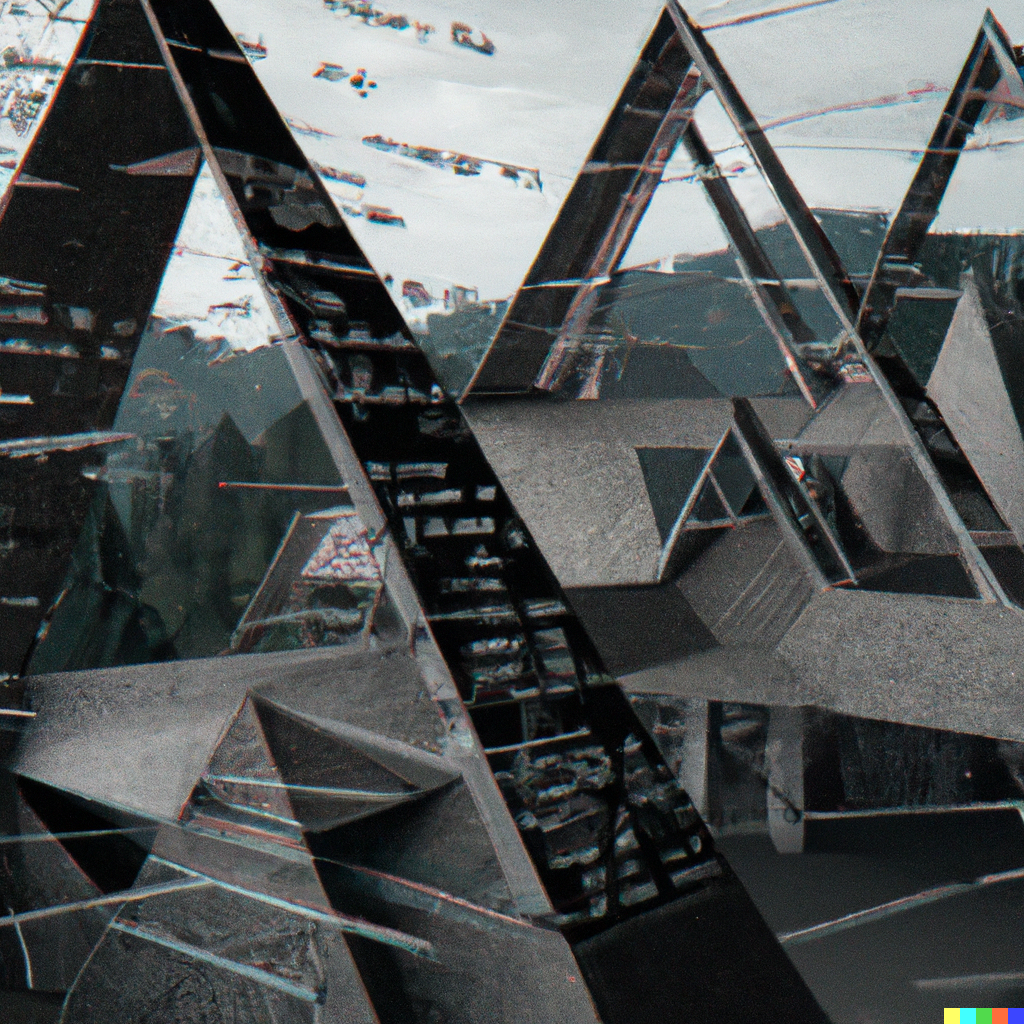
\includegraphics[width=22em]{FallingRoofs2.png}
	\end{center}
	\end{frame}
}

\begin{frame}[allowframebreaks]
	\begin{thebibliography}{9}
		\bibitem{Boole} G.~Boole, \textsl{An Investigation into the Laws of Thought} (1854).
		\bibitem{Grobner} D. Cox, J. Little, D. O'Shea, \emph{Ideals, Varieties, and Algorithms} Fourth Edition, Springer (2015).
		
		\bibitem{girard_llogic}
		J.-Y.~Girard, \textsl{Linear Logic}, Theoretical Computer Science 50 (1), 1--102 (1987).
		
		\bibitem{Girard} J.-Y.~Girard, \emph{Multiplicatives}, Logic and Computer Science: New Trends and Applications. Rosenberg \& Sellier. pp. 11–34 (1987).
		
		\bibitem{towards_goi}
		J.-Y.~Girard, \textsl{Towards a geometry of interaction}, In J.~W.~Gray and A.~Scedrov, editors, Categories in Computer Science and Logic, volume 92 of Contemporary Mathematics, 69--108, AMS (1989).
		
		\bibitem{bs}
		J.-Y.~Girard, \textsl{The Blind Spot: lectures on logic}, European Mathematical Society, (2011).
		
		\bibitem{proofstypes}
		J.-Y.~Girard, Y.~Lafont, and P.~Taylor, \textsl{Proofs and Types}, Cambridge Tracts in Theoretical Computer Science 7 ,Cambridge University Press (1989).
		
		\bibitem{howard} W.~A.~Howard, \textsl{The formulae-as-types notion of construction}, in Seldin and Hindley \textsl{To H.B.Curry: essays on Combinatory logic, Lambda calculus and Formalism}, Academic press (1980).
		
		\bibitem{Laurent} O. Laurent, \emph{An Introduction to Proof Nets}, \url{http://perso.ens-lyon.fr/olivier.laurent/pn.pdf} (2013).
		
		\bibitem{murfet_ll}
		D.~Murfet, \textsl{Logic and Linear Algebra: An Introduction}, preprint \url{https://arxiv.org/abs/1407.2650v3} (2017).
		
		\bibitem{gmz} D.~Murfet and W.~Troiani, \textsl{{G}entzen-{M}ints-{Z}ucker duality}, preprint \url{https://arxiv.org/abs/2008.10131} (2020).
		
		\bibitem{Troiani} W. Troiani, \emph{Linear logic}, lecture notes \url{https://williamtroiani.github.io/MathNotes/LinearLogic.pdf} (2020).
		
		\bibitem{cut_operation} D. Murfet, \emph{The cut operation on Matrix Factorisations} \url{https://arxiv.org/abs/1402.4541}
		
		\bibitem{elimination} D. Murfet, W. Troiani, \emph{Elimination and cut-elimination in multiplicative linear logic} \url{https://arxiv.org/abs/2207.10871?context=cs.LO}
		\end{thebibliography}
	\end{frame}
	
\end{document}